\chapter{Tree Implementation} % Write in your own chapter title
\label{Chapter6}
\lhead{Chapter 6. \emph{Tree Implementation}}

\section{Methodology}
Balanced trees are used to carryout basic operation on the data array. These basic operations and their working are as follows:

	\subsection{Insertion}
	Id's of employees are used to populate the self-balancing binary search tree i.e.,\textit{ AVL trees} and then data is linked with the corresponding nodes. Tree is balanced by the phenomenon of left, right, left-right and right-left rotations.
	
	Time Complexity: \textbf{O(log N)} \\
	Space Complexity: \textbf{O(N)}
	
	\subsection{Finding}
	In AVL trees the nodes are arranged in specfic order. Left child node always have key less than the root node and right child will have key greater than the root node. So finding a tree node involves comparing the "key to be found" at each node if its less then only traverse the left subtree and if its larger then traverse the right subtree. In our case we found the even indexed records from data array in tree and measured its execution time and memory consumption.
	
	Time Complexity: \textbf{O(log N)} \\
	Space Complexity: \textbf{O(N)}
	
	\subsection{Sorted Traversal}
	Due to the order propety of AVL trees sorting traversal can be done simply by \textit{inorder traversal} of the tree. In order traversal involves first traversing the left sub-tree recursively then visiting the root node and finally right sub-tree is traversed recursively.
	
	Time Complexity: \textbf{O(N)}   \textit{Note: This time complexity is only for traversal}\\
	Space Complexity: \textbf{O(N)}
	
	\subsection{Deletion}
	Deletion is carried out by going to the tree node to be deleted and then finding the minimum key or element in its right subtree and replacing the node's key with this minimum key. In this way, the order of AVL tree is maintained. In this engineering problem, we deleted all the odd indexed records from the tree.
	
	Time Complexity: \textbf{O(log N)} \\
	Space Complexity: \textbf{O(N)}
	
\section{Execution Times and Memory Consumptions}
\begin{figure}[H].
	\centering
	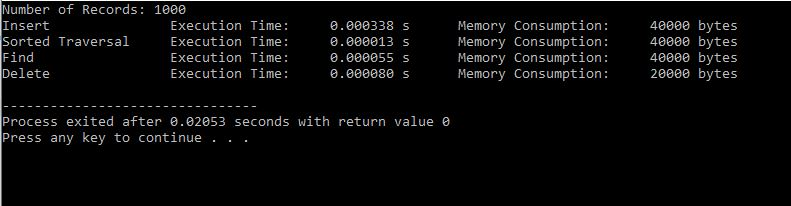
\includegraphics[scale =0.7]{./Figures/Tree1000.jpg}
	\rule{35em}{0.5pt}
	\caption{Results for tree implementation with data size 1000.}
	\label{fig:Tree 1000}
\end{figure}

\begin{figure}[H]
	\centering
	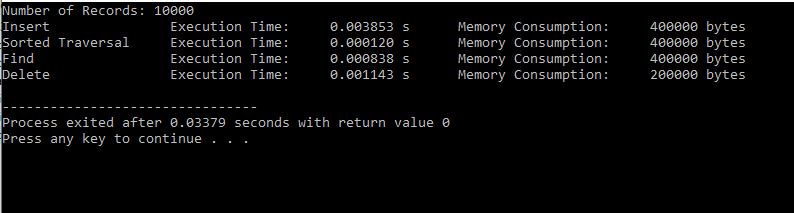
\includegraphics[scale =0.7]{./Figures/Tree10000.jpg}
	\rule{35em}{0.5pt}
	\caption{Results for tree implementation with data size 10000.}
	\label{fig:Tree 10000}
\end{figure}

\begin{figure}[H]
	\centering
	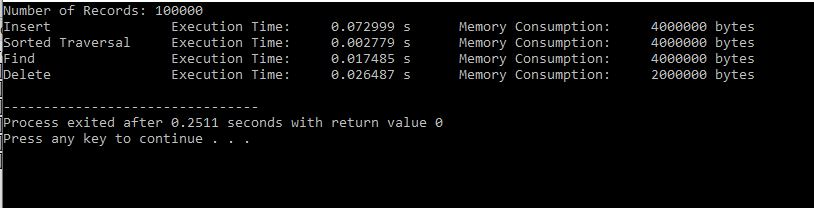
\includegraphics[scale =0.7]{./Figures/Tree100000.jpg}
	\rule{35em}{0.5pt}
	\caption{Results for tree implementation with data size 100000.}
	\label{fig:Tree 100000}
\end{figure}

\begin{figure}[H]
	\centering
	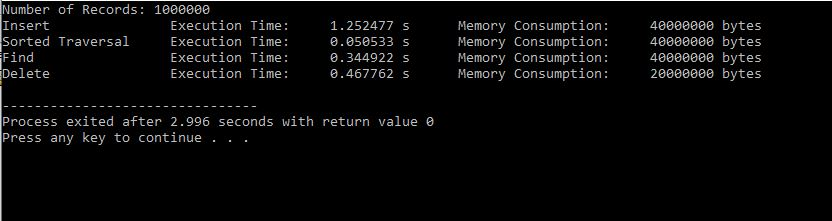
\includegraphics[scale =0.7]{./Figures/Tree1000000.jpg}
	\rule{35em}{0.5pt}
	\caption{Results for tree implementation with data size 1000000.}
	\label{fig:Tree 1000000}
\end{figure}
